%15 min preso!
\documentclass[xcolor=table,aspectratio=169]{beamer}
\usepackage{beamerthemesplit}
\usepackage{wrapfig}
\usetheme{SPbGU}
\usepackage{pdfpages}
\usepackage{amsmath}
\usepackage{cmap}
\usepackage[T2A]{fontenc}
\usepackage[utf8]{inputenc}
\usepackage[english]{babel}
\usepackage{indentfirst}
\usepackage{amsmath}
\usepackage{tikz}
\usepackage{multirow}
\usepackage[noend]{algpseudocode}
\usepackage{algorithm}
\usepackage{algorithmicx}
\usepackage{fancyvrb}
\usepackage{hyperref} 
\usetikzlibrary{calc}
\usetikzlibrary{shapes, backgrounds}
\usetikzlibrary{arrows,automata}
\usetikzlibrary{positioning}
\usetikzlibrary{fit}
\usetikzlibrary{shapes.callouts}
\usetikzlibrary{shapes.misc}
\usepackage{xparse}
\usepackage{fontawesome}

\usepackage{etoolbox,refcount}
\usepackage{multicol}

\usepackage{tabularx}
\newcolumntype{Y}{>{\raggedleft\arraybackslash}X}

\renewcommand{\thealgorithm}{}

\newtheorem{mytheorem}{Theorem}
\renewcommand{\thealgorithm}{}

\newcommand{\tikzmark}[1]{\tikz[overlay,remember picture] \node (#1) {};}
\def\Put(#1,#2)#3{\leavevmode\makebox(0,0){\put(#1,#2){#3}}}

\newcommand{\ltz}{$< 1$}

\tikzset{
    state/.style={
           rectangle,
           rounded corners,
           draw=black, very thick,
           minimum height=2em,
           inner sep=2pt,
           text centered,
           },
}

\tikzset{
    invisible/.style={opacity=0,text opacity=0},
    visible on/.style={alt=#1{}{invisible}},
    alt/.code args={<#1>#2#3}{%
      \alt<#1>{\pgfkeysalso{#2}}{\pgfkeysalso{#3}} % \pgfkeysalso doesn't change the path
    },
}

\tikzset{cross/.style={cross out, draw=black, minimum size=2*(#1-\pgflinewidth), inner sep=0pt, outer sep=0pt, ultra thick},
%default radius will be 1pt. 
cross/.default={1pt}}

\NewDocumentCommand{\mycallout}{r<> O{opacity=0.8,text opacity=1} m m m}{%
\tikz[remember picture, overlay]\node[align=center, fill=cyan!20, text width=#5cm,
#2,visible on=<#1>, rounded corners,
draw,rectangle callout,anchor=pointer,callout relative pointer={(290:0.5cm)}]
at (#3) {#4};
}

\NewDocumentCommand{\mycalloutR}{r<> O{opacity=0.8,text opacity=1} m m m}{%
\tikz[remember picture, overlay]\node[align=center, fill=cyan!20, text width=#5cm,
#2,visible on=<#1>, rounded corners,
draw,rectangle callout,anchor=pointer,callout relative pointer={(30:0.8cm)}]
at (#3) {#4};
}


%callout relative pointer={(230:0.5cm)}]

\newcounter{countitems}
\newcounter{nextitemizecount}
\newcommand{\setupcountitems}{%
  \stepcounter{nextitemizecount}%
  \setcounter{countitems}{0}%
  \preto\item{\stepcounter{countitems}}%
}
\makeatletter
\newcommand{\computecountitems}{%
  \edef\@currentlabel{\number\c@countitems}%
  \label{countitems@\number\numexpr\value{nextitemizecount}-1\relax}%
}
\newcommand{\nextitemizecount}{%
  \getrefnumber{countitems@\number\c@nextitemizecount}%
}
\newcommand{\previtemizecount}{%
  \getrefnumber{countitems@\number\numexpr\value{nextitemizecount}-1\relax}%
}
\makeatother    
\newenvironment{AutoMultiColItemize}{%
\ifnumcomp{\nextitemizecount}{>}{3}{\begin{multicols}{2}}{}%
\setupcountitems\begin{itemize}}%
{\end{itemize}%
\unskip\computecountitems\ifnumcomp{\previtemizecount}{>}{3}{\end{multicols}}{}}


\beamertemplatenavigationsymbolsempty

\title[Анализ данных и формальные языки]{Анализ данных с применением теории формальных языков}
\institute[СПбГУ]{
Санкт-Петербургский Государственный Университет
}

% То, что в квадратных скобках, отображается в левом нижнем углу.
\author[Семён Григорьев]{Семён Григорьев}

\date{2 апреля 2025}


\begin{document}
{
\begin{frame}[fragile]
  \begin{table}
  \centering
  %
\includegraphics[height=1.5cm]{pictures/SPbGU_Logo.png}
  \begin{tabularx}{\linewidth}{XcX}
    %
\includegraphics[height=0.9cm]{pictures/hu_logo.jpeg} 
    \hfill
    & 
    & \hfill 
\includegraphics[height=1.6cm]{pictures/SPbGU_Logo.png}
  \end{tabularx}
  \end{table}
  \titlepage
\end{frame}
}

\begin{frame}[fragile]
  \frametitle{Область интересов}
  
    \begin{itemize}
      \begin{minipage}{0.65\textwidth}
      \item Поиск путей в графах с метками на рёбрах с использованием формальных языков в качестве ограничений\footnotemark
      \begin{itemize}
        \item Регулярные языки (Regular path querying, RPQ): графовые базы данных, часть языка GQL, SMT-решатели
        \item Контекстно-свободные языки (Context-free path querying, CFPQ, CFL-r): графовые БД, статически анализ кода
      \end{itemize} 
    \end{minipage}~  
    \begin{minipage}{0.3\textwidth}
      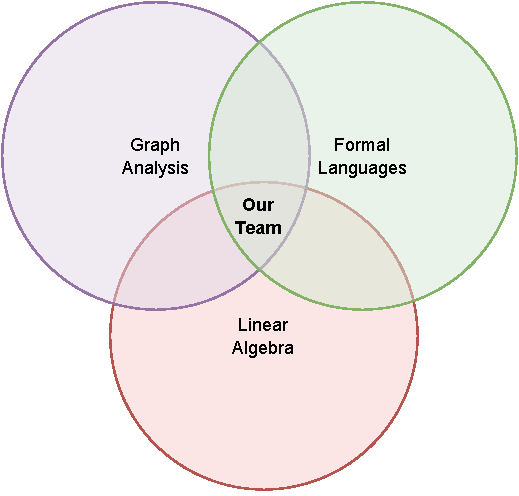
\includegraphics[width = 0.9\textwidth]{pictures/ResearchArea.drawio.pdf}
    \end{minipage}  
      \item Высокопроизводительный анализ графов с использованием линейной алгебры
      \begin{itemize}
        \item Разработка алгоритмов на основе линейной алгебры
        \item Разработка библиотек линейной алгебры, в том числе, с использованием GPGPU
        \item Создание специализированных решений для разработки оптимизации алгоритмов на основе линейной алгебры
      \end{itemize}
    \end{itemize} 
  \footnotetext{Для языка $\mathcal{L}$ и графа с метками на рёбрах $\mathcal{G}$ построить $R=\{ \pi \mid \pi \text{ --- путь в }\mathcal{G}, \omega(\pi) \in \mathcal{L}\}$,
  $\omega(v_0 \xrightarrow{l_0} v_1 \xrightarrow{l_1} v_2 \ldots) = l_0 l_1 \ldots$} 
\end{frame}

\begin{frame}[fragile]
  \frametitle{Формальные языки как ограничения на пути\footnote{Наше сообщество на GitHub: \url{https://github.com/FormalLanguageConstrainedPathQuerying}}: алгоритмы}
  \begin{itemize}
      \item[\faCheck] Диссертация Рустама Азимова про CFPQ с использованием линейной алгебры
      \item[\faCheck] Оптимизации CFPQ (Владимир Кутев, Илья Муравьев, Егор Орачев, Арсений Терехов и многие другие)
      \item[\faCheck] Базовая версия CFPQ LAGraph\footnote{\url{https://github.com/GraphBLAS/LAGraph/pull/265}} (Ильхом Комбаев)
      \item[\faCheck] Базовая версия RPQ LAGraph\footnote{\url{https://github.com/GraphBLAS/LAGraph/pull/261}} (Георгий Белянин)
      \item[\faGears] Перенести в LAGraph различные вариации алгоритмов CFPQ и RPQ и их оптимизации
      \item[\faGears] Диссертация Ольги Бачище про CFPQ с использованием обобщённого LL алгоритма
      \item[\faGears] Интеграция алгоритмов в инструменты статического анализа кода
  \end{itemize}
\end{frame}

\begin{frame}[fragile]
  \frametitle{Формальные языки как ограничения на пути: сопутствующие материалы}
  \begin{itemize}    
    \item Расширение курса по теории формальных языков (Вадим Абзалов, Екатерина Шеметова, Екатерина Вербицкая, Егор Орачев, Николай Пономарев, Ефим Кубышкин, и многие другие)
      \begin{itemize}
        \item[\faCheck] Задачи, система проверки\footnote{\url{https://github.com/FormalLanguageConstrainedPathQuerying/formal-lang-course}}
        \item[\faGears] Разрабатывается конспект лекций\footnote{\url{https://github.com/FormalLanguageConstrainedPathQuerying/FormalLanguageConstrainedReachability-LectureNotes}}
      \end{itemize}
    \item Набор данных\footnote{CFPQ\_Data: \url{https://github.com/FormalLanguageConstrainedPathQuerying/CFPQ_Data}}
    \begin{itemize}
      \item[\faGears] Интеграция в SuiteSparse matrix  collection
    \end{itemize}
  \end{itemize}
\end{frame}


\begin{frame}[fragile]
  \frametitle{Линейная алгебра и анализ графов\footnote{Наше сообщество на GitHub: \url{https://github.com/SparseLinearAlgebra}}}
  \begin{itemize}
    \item Линейная алгебра на GPGPU (Егор Орачев, Владимир Кутуев, Дмитрий Козенко и многие другие)
    \begin{itemize}
      \item[\faCheck] cuBool\footnote{\url{https://github.com/SparseLinearAlgebra/cuBool}}: разреженная булева линейная алгебра на Cuda
      \item[\faCheck] Spla\footnote{\url{https://github.com/SparseLinearAlgebra/spla}}: обобщённая разреженная линейная алгебра на OpenCL
      \item[\faGears] Перенос Spla на RISC-V
    \end{itemize}
    \item Вклад в экосистему GraphBLAS
    \begin{itemize}
      \item[\faCheck] Векторизация умножения матриц на RISC-V RVV1.0\footnote{Реквест с изменениями: \url{https://github.com/DrTimothyAldenDavis/GraphBLAS/pull/381}} (Родион Суворов) 
      \item[\faGears] Кросс-сборка
    \end{itemize}
    \item[\faGears] Эксперименты с RISC-V GPGPU Vortex (Даниил Власенко)
  \end{itemize}
\end{frame}

\begin{frame}[fragile]
  \frametitle{Средства разработки и оптимизации}
  \begin{itemize}
    \item[\faGears] Brahma.FSharp\footnote{\url{https://github.com/YaccConstructor/Brahma.FSharp}}: программирование GPGPU с использованием F\#/.Net
    \item[\faGears] GraphBLAS-sharp\footnote{\url{https://github.com/SparseLinearAlgebra/GraphBLAS-sharp}}: обобщённая разреженная линейная алгебра в функциональном стиле (Игорь Ерин, Кирилл Гарбар, и многие другие)
    \begin{itemize}
      \item Как решить проблему неявных нулей?
      \item Можно ли упростить GraphBLAS API?
    \end{itemize}
    \item[\faGears] LamaGraph\footnote{\url{https://github.com/Lamagraph/interaction-nets-in-fpga}}: программно-аппаратный комплекс для ускорения обобщённой разреженной линейной алгебры (Николай Пономарев, Ефим Кубышкин)
  \end{itemize}
  
\end{frame}

\begin{frame}[fragile]
  \frametitle{Разное}
  \begin{itemize}
    \item Графовые нейронные сети и символьное исполнение
    \begin{itemize}
      \item PySymGym\footnote{\url{https://github.com/PySymGym/PySymGym}}: инфраструктура для обучения нейронных сетей управлению символьной машиной (Анна Чистякова, Давид Ахмедов, Данил Парфёнов, и многие другие)
    \end{itemize}
    \item Биоинформатика (Анна Чистякова, Полина Лунина, Юлия Сусанина)
    \begin{itemize}
      \item Предсказание вторичной структуры РНК
      \item Анализ метагеномных сборок
    \end{itemize}
    
  \end{itemize}
\end{frame}


\end{document}
